\section{Main contributions}\label{contributions}
The main contribution of this thesis is the theoretical foundation of a new approach to UI development with a UI framework. A proof of concept demonstrates the major theoretical contributions. On a larger scale this thesis contributes to the fight against accidental complexity in software development.

\subsection{Methods}\label{usecases}
We chose to follow a process including the following points in order to explore possible answers and solutions to the thesis.

\paragraph{Use of scores}
In order to evaluate the UI framework and its concepts we are using two scoring systems. To asses whether goals have been met scores between 0 and 3 are used. To gauge how complexity has been effected we use scores between -3 and 3.

\begin{table}[]
  \begin{center}
    \begin{tabular}{|c|l|}
      \hline
      Score & Effect on goal \\
      \hline
      0 & Goal not met \\
      1 & Slight improvement towards goal \\
      2 & Goal mostly met \\
      3 & Goal completely fulfilled \\
      \hline
    \end{tabular}
    \caption{Scores to evaluate whether goals have been met}
  \end{center}
\end{table}

\begin{table}[]
  \begin{center}
    \begin{tabular}{|c|l|}
      \hline
      Score & Effect on complexity \\
      \hline
      -3 & Massive increase in complexity \\
      -2 & Increase in complexity \\
      -1 & Slight increase in complexity \\
      0 & No change in complexity \\
      1 & Slight decrease in complexity \\
      2 & Decrease in complexity \\
      3 & Massive decrease in complexity \\
      \hline
    \end{tabular}
    \caption{Scores to gauge the change in complexity}
  \end{center}
\end{table}

\paragraph{Conceptual analysis of user interfaces}
Through analysis of the typical usage patterns of user interfaces we can derive coarse business requirements of the UI framework. These serve as foundation for further requirements engineering.

\paragraph{Definition of major design goals}
Major design goals of the UI framework are directly influenced by non-functional requirements. We consider the broader scope of UI development in order to obtain those. This includes analysis of:

\begin{enumerate}
  \item the development process of UIs with web technologies
  \item contemporary frameworks and tools for UI development that enjoyed wide and rapid adoption
  \item contemporary frameworks and tools for UI development that failed
\end{enumerate}

By following what tools in \textbf{2} did right and avoiding the mistakes of tools in \textbf{3}, we define a set of design goals that the proof of concept should adhere to.

\paragraph{Definition of the proof of concept}
The section defines the artifact that can be used to create UIs. The proof of concept should demonstrate the viability of the thesis.

\paragraph{Definition of the development process}
The proof of concept is a software artifact and is developed with respect to current engineering best practices.

\paragraph{Definition of real world use cases}
By defining real world applications for the UI framework, we discover user roles and user stories.

\paragraph{Implementation of proof of concept driven by use cases}
The UI framework is developed incrementally use case by use case. The major design goals are respected.

\paragraph{Evaluation of design goals}
We analyze the design goals and whether they have been met. The design goals are not equally important, so they get a weight assigned. We assess each design goal qualitatively and assign a score between 0 and 3.

The mean of all scores is calculated to asses whether the design goals have been met.

\paragraph{Conclusion of approach to reduce Accidental and Essential Complexity}
We break up software complexity into more specific types of complexities. Software complexity comprises Essential Complexity and Accidental Complexity according to Brooks. Essential Complexity has several causes on its own.

After identifying types of complexity, we asses how the UI framework affects them by assigning a score between -3 and 3.

\subsection{Conceptual analysis of user interfaces}
For a system to be useful, it has to interact with its environment. These interactions happen through multiple types of interfaces, which are used by two types of users. The users are either other systems or human users.
The interfaces for human users (user interfaces) have typical characteristics,
By observing the usage of a user interface by the user we can analyze the main characteristics. A typical scenario of UI usage is browsing a website. What does the user do while browsing a website? It is typically one of two things: he either reads or clicks.

\textbf{Reading} a website is equivalent to data \textbf{querying}. The user \textbf{querying} data

The usage of a UI by a user consists of either \textbf{reading} or \textbf{interacting}. In terms of systems we can call them \textbf{querying} or \textbf{interacting} respectively.
\begin{enumerate}
  \item Query: The user is able to retrieve information from the UI by looking at it
  \item Interacting: The user is able to interact with the UI
\end{enumerate}

The development of the UI framework is driven by the implementation of these two capabilities.

\subsection{Design goals}
Following design goals should be met by the UI framework. For each design goal we discuss the goal itself and the reason behind it, how we intend to meet it and how it can be measured.

\subsubsection{Play nicely with others}\label{usecases}
The most important design goal is to play nicely with others. It is important to respect standards and keep compatibility with existing tooling. This design goal drove the choice of JSON-LD as serialization format for linked data.

We acknowledge the widespread use of HTTP and JSON as data exchange format and achieve this design goal by conforming to web standards and \textbf{extending} existing tooling. JSON-LD allows us to stay compatible with all tools consuming and producing JSON.

This design goal can be quantified by analyzing each component of the UI framework and determine whether the technologies, protocols, languages and tools for that component are either formally standardized or a defacto standard.

\subsubsection{Straightforward upgrade path}\label{usecases}
In order to help the adoption of the UI framework it is important to show a clear upgrade path and to keep the friction at a minimum.

This can be achieved by \textbf{extending} existing standards, keep breaking changes at a minimum and with good documentation. Playing nicely with others helps to reach this design goal as well.

This design goal can be quantified by measuring or estimating the effort that needs to be spent to upgrade a conventional API to the suggested hypermedia API.

\subsubsection{Customizability}\label{usecases}
While providing sane defaults, the UI framework should be customizable. There should be no limitations imposed in terms of what UIs can be drawn.

We want to achieve this goal be allowing the UI developer to override the sane defaults. The UI developer can decide to completely ignore the linked data aspect and consume the HTTP API in a traditional way by hard coding knowledge into the client. The use of React as UI library allows the UI developer to pull in external React components.

This design goal is met if all possible UIs that can be drawn with conventional tools can be drawn using the UI framework. By allowing the UI developer to consume the hypermedia API as conventional API this goal is met.

\subsubsection{Developer ergonomics}\label{usecases}
The UI developer should be able to use the UI framework with spending minimal effort on learning.

This goal can be achieved by choosing a widely used platform that has a striving open source community. It is important that there is an open source community working on that platform because a wide adoption behind closed doors is less likely to improve developer ergonomics.
A big market share of the platform increases the chances that the developer is already familiar with it. The tooling of these platforms tends to be polished and battle tested. The developer is less likely to get stuck because of some edge case issues.

An established and widely adopted platform is Node and the NPM (Node Package Manager) ecosystem. This is the platform that we choose to develop the UI framework in.

\subsection{Proof of concept}
I define two real-world use cases that cover the two main capabilities of \textbf{rendering data} and \textbf{user interaction}. Each of those use cases are split up into user stories that can be implemented separately. This ensures that the design goals are met and all user roles are considered.

\subsection{Use Case 1: Apartment}\label{usecases}
For the user to be able to query data the UI has to render it.

The first use case describes a scenario in home automation. Several thermometers in several rooms in an apartment send the current temperature to a server. The goal is to develop a UI that displays apartments, rooms, and thermometers and temperatures in a sensible manner.

\begin{figure}[!htb]
  \center{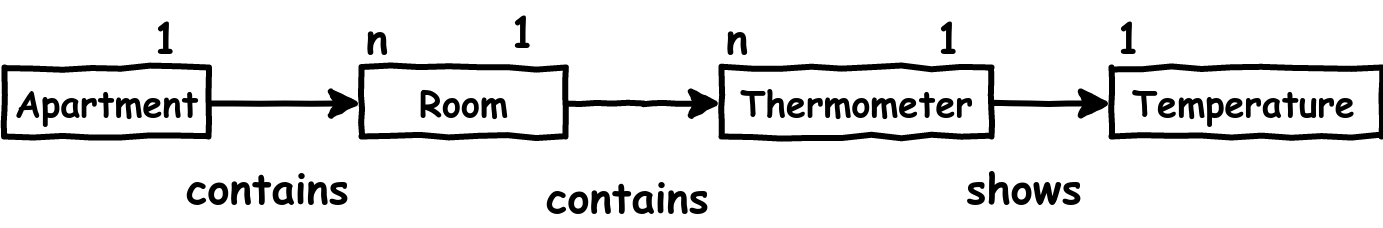
\includegraphics[width=100]
    {images/iot.png}}
  \caption{\label{fig:my-label} Data model of the kanban board use case.}
\end{figure}

\begin{table}
  \begin{center}
    \begin{tabular}{ |c|l| }
      \hline
      ID & Story title \\
      \hline
      S01 & As landlord I want to overview my apartments \\
      S02 & As landlord I want to overview all rooms of an apartment \\
      S03 & As landlord I want to overview thermometers of room \\
      S04 & As landlord I want to overview the measurement data of a thermometer \\
      S05 & As UI developer I want to present all available data without spending any development time \\
      S06 & As UI developer I want to be able to customize the UI in order to improve it incrementally \\
      \hline
    \end{tabular}
    \caption{User stories of a client that consumes a home automation API}
  \end{center}
\end{table}

\subsubsection{Base hypermedia vocabulary}\label{basevocab}
\subsubsection{UI rendering}\label{genericrendering}
This paragraph focuses on presentation of data by rendering UI components in the context of web development.
\subsubsection{Leveraging linked data for UI rendering}\label{linkeddatarendering}
\subsubsection{From JSON-LD to domain rendering}\label{domainrendering}

\subsection{Use Case 2: Kanban Board}\label{usecases}

\begin{figure}[!htb]
  \center{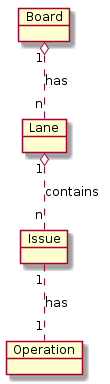
\includegraphics[width=100]
    {images/kanban.png}}
  \caption{\label{fig:my-label} Data model of the home automation use case.}
\end{figure}

\begin{table}
  \begin{center}
    \begin{tabular}{ |c|l| }
      \hline
      ID & Story title \\
      \hline
      S01 & As project manager I want to overview all projects \\
      S02 & As project manager I want to overview all issues of a project \\
      S03 & As project manager I want to see the status of an issue \\
      S04 & As project manager I want to change the status of an issue \\
      S05 & As project manager I want to create new issues \\
      S06 & As project manager I want to remove issues \\
      S07 & As UI developer I want to present all available data without spending any development time \\
      S08 & As UI developer I want to be able to customize the UI in order to improve it incrementally \\
      S09 & As UI developer I want to expose all operations to the project manager without spending initial effort \\
      \hline
    \end{tabular}
    \caption{User stories of a simple software project management tool}
  \end{center}
\end{table}

\begin{figure}[!htb]
  \center{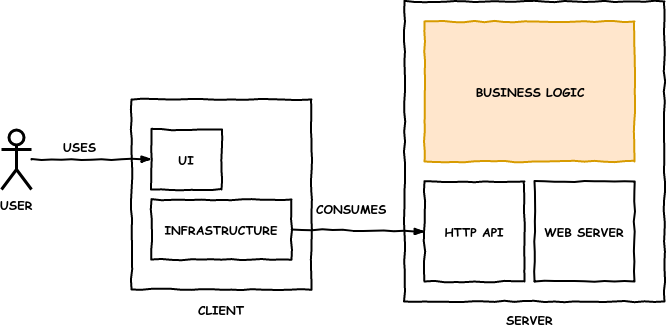
\includegraphics[width=380]
    {images/ui-dev.png}}
  \caption{\label{fig:my-label} Solely the server contains business logic.}
\end{figure}

\begin{figure}[!htb]
  \center{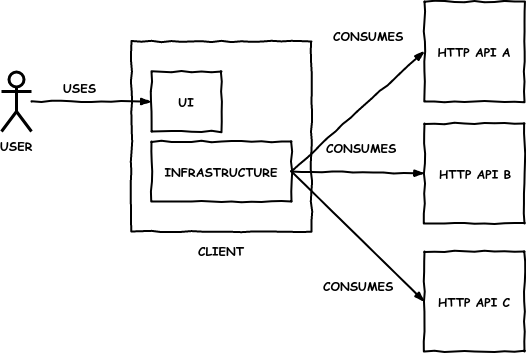
\includegraphics[width=380]
    {images/client-instances.png}}
  \caption{\label{fig:my-label} The client is decoupled from any API and is able to consume different APIs.}
\end{figure}

\begin{figure}[!htb]
  \center{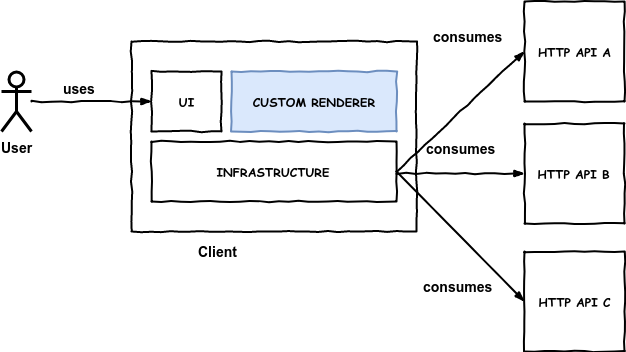
\includegraphics[width=380]
    {images/ui-dev-custom-renderer.png}}
  \caption{\label{fig:my-label} Custom renderers provide the ability to render linked data types. By avoiding hard coding business logic into the client the coupling to the server is still lose.}
\end{figure}

\subsubsection{Task based computing}\label{interaction}

\subsubsection{User interaction}\label{interaction}

TODO three types of operations:

inline operations
supported operations for all of the resource's types
supported operations for the supported property, where the resource is an object of said property

\subsubsection{CQRS}\label{interaction}
